\documentclass[12pt]{article}
\usepackage{hyperref}
\usepackage{notoccite}
\usepackage[backend=biber, sorting=none, style=ieee]{biblatex}
\author{Elliot Lake}
\usepackage{lscape}
\usepackage{graphicx}
\usepackage{geometry}
\title{Multiple Objective Evolutionary Algorithms For Narratives Through the Lens of Spiritual Theology}
\graphicspath{ {./Charts/} }


\addbibresource{bigbib.bib}

\begin{document}
\maketitle
\pagebreak 
\section{Abstract}
While Narrative Generation has focused much on plot generation, this has been to the neglect of nuanced characters in some cases. One approach to alleviating this problem is to take inspiration from studies on human action and nature. An otherwise unacknowledged approach to this is the venerable Catholic Spiritual Tradition, which articulates the progression in life of those who live the Christian Life. This thesis aims to implement a partial representation of that life computationally. To aid this, an Indicator-Based Multiple Objective Evolutionary Algorithm (MOEA)was written to rank these lives in line with Catholic Spiritual Teaching on the structure of the Spiritual Life. Although we have found, based on tentative data, that these characters are less realistic than hoped, those tested found those characters entertaining. Additional work to be done could be the investigation of Hagiographic Literature and other aspects of the tradition.
\section{Acknowledgements}

I would like to thank my project supervisor Dr Anna Jordanous for helping me a great deal with the breadth of her knowledge of computational creativity literature and for her enthusiasm for this project. \\

I would also like to thank my friends, in particular Sebastian Damrath, whose input as an experienced Software Developer has made this and a lot of other things possible.

I would like to finally and especially all of those people who filled out my survey. If you didn't sacrifice your time to assist me in this work, it would not have been possible to determine to any extent whether it was operable or not. 

\pagebreak
\tableofcontents


\section{Introduction}
Since the 1960s, thousands of projects and many innovations have occurred in the field of narrative generation. From new software able to produce ever more complicated and interesting plots, through to substantial translations of narrative theory to computational models, much has been accomplished. However, a common occurrence with these solutions is that much attention has been paid to the technicalities of good plots, while very little time has been spent making characters that are nuanced. In some cases, such as folktales, intentionally stereotyped characters have been employed, which while this serves the intent of folktales, doesn't encompass the full range of human behaviour. Simultaneously, this field is seemingly unaware of thousands of years of writings that articulate precisely this nature. This is encapsulated by the thousands of authors in the Roman Catholic Spiritual and Moral Tradition, often in straightforward, detailed and analytical manuals. This could be an excellent resource for the design of characters, as what makes stories relevant is their imitation of reality and their readability. Under these manuals especially, habits are described as virtues and vices, and emotions as passions. These habits are then divided down into subvirtues and subvices. This rigid delineation of human habits, and how they pertain to human nature, significantly reduces the difficulty in computerising the facets of this nature, which is often very hard to consider through a purely quantitative system such as a Computer.  \\

One way of managing these values, while maximising them, is through Genetic Algorithms. Genetic Algorithms are present in Narrative Generation literature and have been used to great effect to improve and evaluate stories, often on the basis of tension. However, there is a seeming lack of Multiple Objective Evolutionary Algorithms (MOEAs). As each character has multiple facets (In our case, we will be using 7 Virtues as described by Thomas Aquinas), optimising each of those values will require a Multiple Objective approach. There are many valid approaches to solving Multiple Objective problems because with multiple values there must be some manner of managing compromises in the values where values don't Pareto Dominate\footnote{I.E. are better in all cases} one another. As these virtues are not ontologically distinct from the person, these methods must take account of the virtues being dependent. \\

Our primary aim with this thesis is to view how effective a partial implementation of Catholic Spiritual Theology computationally can be for generating characters that are realistic and entertaining. Secondarily, we wish to observe how effective MOEAs are in helping us to achieve this aim. \\ 
\section{Literature Review}
As narrative theory and generation are broad fields with a great deal of literature in each, we must break down and elaborate upon relevant research in each area so that subsequent explanations of approaches and implementation are intelligible.

\subsection{Current Use of Narrative Theory in Narrative Generation}
There have been human narratives for as long as there have been humans, but Narrative Theory is a much newer beast. The earliest instance of Narrative Theory we have was written in the 4th Century BC by Aristotle. This was called the Poetics. This tradition has been built upon by many authors up until the present, and these are often utilised by authors working in Narrative Generation.  For instance, Freytag's Pyramid is used in at least one Narrative Generation paper which generates quests for video games\cite{questgeneration}.  Freytag's Pyramind is a narrative structure developed during the 19th Century by Playwright Gustav Freytag. Likewise, more implicit traditions of folk storytelling have been very influential. For example, \cite{MEXICA} is a story generation system that is based on the Narrative Tradition of the Mexica people. More prominently, the famous Propp Grammar which seems to be almost omnipresent in Narrative Generation literature. This is based on a collection of aspects of Russian Folk Tales \cite{propp1975morphology}. Similar work has also been done for Western African Traditions \cite{WestAfricanGeneration} and for many more.  There have even been efforts to computerise Propp's Grammar directly.\cite{Gervs2013ProppsMO}. These investigations have gone a long way towards representing human thought, including ethical and teleological concepts, manifest through Computer Systems. \\

\subsection{Virtue Ethics, Human Nature and Spiritual Theology}
However, an overwhelming amount of emphasis is placed on the Plot in these projects, to the extent that characters suffer. In many of these Story Grammars and Traditions, characters lack the nuances of human behaviour. However, there is an immense wealth of theoretical work, wherein the aim is to articulate human behaviour, which could be used to remedy this issue. Beginning somewhere between the 15th and 13th Centuries BC, the Abrahamic Tradition, especially in dialogue with the Greek Philosophical Tradition, has generated a dizzying array of texts investigating the nature of man, what man ought to do, what he ought not to do and articulating his development throughout life. This could provide us with a great theoretical toolset for articulating characters, which to the best of my knowledge has been entirely overlooked. \\

Besides the Old and New Testaments themselves, the Nicomachean Ethics \cite{340BCEthicsAristotleNicomachean} is one of the first systematic treatments of Human Virtue\footnote{In this case referring to the proper function of human functions, when aimed towards an objective good which fits this}. A few hundred years later, the Catholic Spiritual and Moral Tradition emerged. Beginning in earnest in the 3rd Century AD with Origen\cite{bergsma2018catholic}, and being further clarified by various patristic authors such as Gregory the Great and Maximus the Confessor, the two traditions began a dialogue in the 8th Century under the pen of John Damascene. This became particularly pronounced in the Scholastic Tradition, which began in the late 11th Century with Anselm of Canterbury, and continues to this day through authors such as Fr Reginald Garrigou-Lagrange, whose towering character as a theologian is best known through his Magnum Opus in Spiritual Theology \: Three Ages of the Interior Life \cite{garrigou2013three}.\\

The uniting theme of the vast majority of these spiritual writings is in those three ages representing stages towards loving union with God. These are known as the Purgative, Illuminative and Unitive ways. Under the Purgative, a person is purged of all chosen moral evil, from murder through to more venial matters like swearing. The vast majority of people never pass this stage. In the Illuminative way, people who persist are enlightened with information and begin to greatly change their aims from natural goods towards the divine good of Charity, which consists in Loving God and Neighbour by choice rather than by emotion. The final stage, the Unitive, focuses on making the person ever closer to God after the obliteration of almost all sins and imperfections. \\ 

This is clearer in later writings than in earlier ones. In comparison to earlier unsystematised spiritual writings, such as those compiled in the Philokalia\cite{1983philokalia}, the Scholastic synthesis produced a large number of vast theological treatises, which are both known for their clarity and their comprehensiveness. A particularly important example of this would be the Summa Theologiae of Thomas Aquinas, which provides an overwhelmingly large summary of Moral Teaching \cite{aquinas2014summa}, which Spiritual Theology relies on. The aforementioned Fr Garrigou-Lagrange also writes in this same manner in the Three Ages of the Interior Life\\.

Up until this point, I am unaware of any attempts in Narrative Generation to replicate a Scholastic, or even broadly Aristotelian, view of man to articulate characters.\\
\subsection{Computational Character Generation}
This same absence of research is felt concerning characters generally in Narrative Generation research. However, there is not a complete absence. As is noted in a survey on Automatic Story Generation \cite{AutomaticStoryGeneration2021}, the emphasis is placed much more on plot generation techniques rather than characters, and even in character-based surveys, only one project gives free rein to characters \cite{Riedl2003CharacterfocusedNP}. However, projects such as MEXICA\cite{MEXICA} give some emphasis to characters while remaining plot dominated.\\

In MEXICA, there are two stages. The first is called Engagement. During Engagement, character actions are determined based on emotional bonds and tensions between characters. There is a collection of story actions that are characterised by Preconditions and postconditions, which are triggered when bonds and tensions are at the correct level. Subsequently, there is another process called Reflection. This utilises insights from studies into human cognition when employed in story-making, which structures these initial stories into something more palatable to an audience. Additionally, in Planning Author and Character Goals for Story Generation \cite{authorandcharactergoals}, while characters are not defined strictly, they are defined in terms of their goals, in this case being concerning children's stories. This motivation drives the plot, which forms the stories. However, one project which defines stories mostly based on characters is Talespin \cite{Meehan1977TALESPINAI}. Talespin operates by taking the aspects of the lives of characters and allows them to produce the stories by acting on their needs and their beliefs, with the aid of an inference engine, which generates subsequent steps based on the goals which emerge from the predicament of the character.  \\  
\subsection{General Approaches to Narrative Generation}
Despite the conspicuous lack of character-focused storytelling, there are a wide array of different methods which have been used for the generation of narratives. These are generally set into 5 general categories described by Kyrbartas\cite{KybartasGenerationTechniques} \: Plot Grammars (as mentioned earlier, and are collections of structures and elements in stories), Planning Based (Which selects goals and builds to them), Interactive, Case-Based (Which incorporates pre-defined aspects into the generation which must be there) and Genetic Algorithms. Additionally, there are also Neural Network approaches which I note here additionally. 

The first three make intuitive sense when there is an approach that involves a plot-first form of generation. After all, when we engage in this the plot is a greater concern than the characters. These methods have been somewhat popular in Narrative Generation. As Narrative Generation in the wild shows \cite{van-stegeren-theune-2019-narrative}, around a quarter of 61 projects used some form of hard narrative planning, and others used means amenable to the aforementioned methods (Markov Chains for Plot Graphs, Templating etc.). Deep Learning, by contrast, had only 3 projects, and simulations were only used 5 times. Neural Network-based approaches tend to work well with simplistic approaches, such as is demonstrated here \cite{NeuralNetworkOne}. However, this approach isn't always effective due to the propensity to produce incoherent stories. As coherence is an important aspect of storytelling \cite{sagarkar-etal-2018-quality}, Neural Network approaches are occasionally overlooked. \\

In stark contrast, Genetic Algorithm based approaches have been shown to be very effective \cite{mcintyre-lapata-2010-plot}, even to the point of slightly exceeding plot grammar (called graph in the paper) and rank based implementations. Genetic algorithms, by their nature, are broadly applicable, and this is shown in this area of study. For instance, Genetic Algorithms can be used in the generation of video game quests \cite{questgeneration}, and are effective to the point of almost approaching the quality of professionally designed quests. Also, they have been used to assist in refining stories into more coherent states. This was the aim of Live, Die, Evaluate, Repeat\cite{Riegl2018LiveDE}. Finally, this approach has even been used in the context of character generation \cite{charactergeneration}, which demonstrated that this can be used effectively to produce a character with varying states. Although less typical in Narrative Generation, there have also been uses of Multiple Objective Evolutionary Algorithms (MOEAs)\cite{MOEANarrative}, and has proven to be effective at improving narrations.
\subsection{MOEAs}
MOEAs have been around for almost as long as Narrative Generation Systems. Multiple Objective problems usually exist because engineers cannot come up with a way to abstract out other aspects into singular variables, and therefore they tend to be more difficult to solve. In a single objective GA, it is very straightforward to discern which results are best based on a single-dimensional score. In cases where results for a Multiple Objective problem are objectively inferior to others, they are referred to as Pareto Dominated solutions. However, this is rarely the case, which makes these inferior to other, more modern approaches to the problem\cite{AchievementScalarazingIndicatorBased}. This necessitated reading into more modern methods. To my surprise, there have been no generation-defining changes in MOEA research since around 2003 \cite{MOEASurvey1}, but despite this, there have been improvements to these algorithms and new algorithms which have emerged, which have proven their effectiveness. MOEA/D, which decomposes Multi-Objective problems down into single objective subproblems \cite{MOEAD} was released in 2007 and has been built on significantly since that initial release. Additionally, there have been innovations in Indicator-Based MOEAs, which operate by producing an indicator score of each potential Pareto Non-Dominated Solutions(which refers to those solutions which are not objectively inferior to other results). From my research, these three categories predominate current MOEA research, and therefore any approaches to balancing Character traits will flow from an algorithm of one of these three types.

\section{Problem Description}
We find ourselves with a complicated problem to solve. Owing to the focus in Narrative Generation research on Plot over Characters, the consequence has been a sacrifice in the humanity and realism of the characters present in some publications. Although these stories may be, on paper, sensible and fit narrative arcs which have been described since Aristotle, this does not mean that the characters are realistic. Likewise, there is an absence of detailed examination of what a human person is, and hence a lack of awareness in the field as to how an object with deep qualities such as a human being can be represented quantitatively by a computer. However, there is literature that can do so effectively. Therefore, the aim of this thesis is to attempt to solve the problem of unrealistic and cliched characters through the computerisation of Catholic Spiritual Theology. \\

\section{Possible Approaches}
This, therefore, leaves us to contemplate the approaches to not only represent realistic human characters but also in terms of a practical implementation of these theories. 
\subsection{Approaches to Character Structure}
To learn the nature of human persons, we need a basis. As we have set out with Spiritual Theology as our point of consideration, we ought to consider the two broad categories of these writings.
\subsubsection{Patristic Approach}
The Patristic or Monastic approach is an approach like that of the Philokalia \cite{1983philokalia}, which is a collection of sayings and moral treatises. This form of wisdom also tends to be held in the form of commentaries and homilies. These documents tend to be pithy, detailed, but generally unsystematised. They tend to be much more aphoristic and poetic than systematic and prosaic philosophical treatises. This approach produces a lot of information that is easy and entertaining to read, as well as articulating a great deal of information about human nature, which could then be taken and implemented into a computational model. However, there are notable disadvantages to this method. Firstly, it would be very difficult to implement on a computational level. This is because it is generally unsystematic, and so it becomes hard to simulate the rules or generalities articulated into a system. Also, there is a great deal of variation. There are three broad schools in the first-millennium AD \: Latin, Greek and Syriac. Each possesses a vastly different approach, Syriac being generally poetic while Latin is more legalistic. It would be very difficult to produce a system with these combined. Finally, much of the useful information is in inconvenient places, such as within letters or within homilies, which makes it time-consuming to research. When they do structure virtues in a somewhat systematic fashion, they tend to vary somewhat. For example, in \cite{1983philokalia}, St John Cassian lists 8 principal vices. On the other hand, St Gregory the Great folds this into 7 vices. Due to the vast scale of the tradition, and a great deal being untranslated, I cannot say how vast the variation is throughout the whole. However, what we do have of this tradition is quite variable and therefore hard to computerise. \\
\subsubsection{Scholastic Approach} 
Alternatively, there is the Scholastic Approach, which took the Patristic Approach and synthesised it with Greek Philosophy, producing a far more unified and easily accessible system of knowledge without losing any of the wisdom of the fathers. Beyond being dryer to read, there is no disadvantage to picking a Scholastic approach, because it solves each of the problems mentioned earlier to some extent. It is almost entirely in the Latin Western Tradition, it is completely systematised, and it is marked by the production of theological manuals with clear delineations marking out where everything is with no ambiguity nor with the taxing labour necessary to extract information amid otherwise unrelated homilies. The Scholastic approach to virtue also generally comes from that which is set down by St Gregory the Great, meaning that there are consistently 7 categories of vices, which are then split down into subvirtues and subvices relating to behaviours that contribute to that overall virtue. We will, for the purposes of this thesis, consider Thomas Aquinas' view of the Virtues \footnote{Justice, Prudence, Temperance, Fortitude, Faith, Hope and Charity}. Also, there is a similar systematisation of emotions, which are called passions. St Thomas Aquinas lists 8 \cite{ThomasAq85:online}, which are often mutually contradictory, and so can be folded into each other as a spectrum in the context of software. The parts could also be meaningfully combined into wholes in cases where abstraction is needed.\\
\subsection{Approaches to Output and General Narrative Structure}
Although we have introduced and explained to some extent the advantages of Evolutionary Algorithms for Narratives, it remains to be seen how these will be implemented. 
\subsubsection{MOEAs for Narrative Events}
One way that MOEAs could be utilised would be to employ them to select story events. For example, a population could be groups of story events forming a plot, a fitness function could generate a score to determine to what degree the story fits the various objectives, and then from there, a new generation is spliced together via mutation and/or crossover to form a new population next generation. An advantage of this approach is that it does go some way towards imitating the previous methods of narrative generation, which focus on the plot. If the plot is a character's life, then the events of that life are plot elements, and therefore this would serve to keep the final story structured. However, the problem with this approach is that, for this to be consistent, all of the characters must be without inherent predispositions to virtues or emotions, which in reality people do have. Therefore it may damage the reality of the generation of the characters. While this has the potential to generate coherent narratives, it does so with some disloyalty to the realism of characters.  \\
\subsubsection{MOEAs for Character Stats} 
Alternatively, Character stats could be mutated. This eliminates the aforementioned problem quite clearly. Characters are now no longer Tabula Rasa and henceforth reflect reality more accurately. However, if this were the case, this would render stories utterly non-interchangeable, as people make choices based on previous habits and inborn predispositions. Therefore, it would be more reasonable to autogenerate stories each time with new stats, but this would render stories indeterminate for each character. Therefore, we could end up with a situation wherein the same character stats could lead to two vastly different stories. This would make for a profoundly unreliable narrative generator. Secondly, as in any case, a character would have hundreds of stats (Even if we take a Scholastic Approach), and we were to engage in any other changes beyond mutations, this would be highly complicated to implement with no guarantee to it directly changing the story. For instance, a character could be crossed over with another across a few virtues, but due to the story being autogenerated each time, this may have no impact whatsoever on what is read. While it makes intuitive sense to do this, it doesn't result in the consistency which a narrative generator ought to have. \\

\subsubsection{MOEAs for Events and Stats} 
We could seek to overcome the flaws in both of these approaches by combining them. In theory, this would retain a level of realism that the previous approaches lack. However, the mutation of the stats would indicate that there would be influences in choices throughout the life, which unless managed very well, would lead to a discordance between the stats of the character and the story which results. This lack of cohesion between the story and stats would directly impact any arc to a character as well. Suppose we crossed over two characters with different lives at various points. Their predispositions would realistically impact the characters in different ways too. One person may develop PTSD from a traumatic event while another person is fine. This could not only completely break the coherence of the life segments, but also it could change the stats themselves differently. These would then be addressed inconsistently by the MOEA. While an ideal approach, practical implementation of this could make characters generated to be even less realistic. \\

\subsection{Approaches to MOEAs in Context}
Besides the employment of MOEAs for certain tasks in Narrative Generation, it also must be considered which approaches for ranking the quality of solutions are to be utilised, with their advantages and disadvantages, because misuse of MOEAs could generate inaccurate or incorrect results.
\subsubsection{Pareto Dominance}
A simple approach would be to carry out Pareto Dominance to generate solutions. This would be simply to subtract away all of the objectively inferior solutions, which are lower on all counts than others. This would produce a Pareto Front of various solutions which differ in magnitude across dimensions. While this is simple, this is not a good approach. Firstly, this becomes highly inefficient across more than 3 Objectives \cite{AchievementScalarazingIndicatorBased}, which we will undoubtedly exceed. Secondly, it provides no means inherently of distinguishing between the quality of Pareto Non-Dominated Results which are left behind, which may lead to remaining results from a generation, while being passable, not capitalising on features we may wish to emphasise in the characters.  
\subsubsection{Decomposition}
Decomposition algorithms, such as MOEA/D \cite{MOEAD}, are a very fast approach because their design is inherently simple. As well as being simple to implement, the approach treats each dimension equally, which means that no variable is unnecessarily buried. However, the issue with a Decomposition centred solution is that the algorithm presupposes that the variables are independent, in such a way which so far as I understand is numerically impossible to correct. As MOEA/D cycles through the objectives, it is required to optimise, it varies out consistent weights across the subproblems, assigning them to each objective in proper sequence. This doesn't work when working with dependent variables, as this technique could misbalance certain variables. For example, Dominican Scholastic approaches to Human Decision Making tend to place Prudence as a predominant virtue in this for all actions. Therefore, this makes virtue generally to some extent dependent on Prudence. Cycling weights between the different virtues and passions couldn't eliminate this issue, because it's not reducible to a set modification of a coefficient. This is made even worse because, as this has no previous research applied to it, that there may be hidden dependent variables which we cannot simply modify the algorithm to deal with.  \\
\subsubsection{Indicator Based} 
However, an indicator based solution could take account of problems of dependent variables if the indicator was able to take this into account. For example, an indicator that operates by distance could take account of a character as a point on a graph, which would mean that the character could be taken as a whole. However, dependent on the indicator function, MOEAs could be a lot slower than a Decomposition based counterpart. As we see with K Nearest Neighbour Clustering Algorithms in Data Mining\cite{CompareML}, these algorithms tend to be a lot slower than others, such as Decision Tree algorithms. This could be the same in our final implementation if this were settled on. \\

\section{Design and Methodology}
To incorporate any approach to investigating the effectiveness of Spiritual Theology, there must be an appropriate degree of orderliness to this endeavour.
\subsection{Methodology}
It would be a poor idea, in a work that is speculative by nature, to structure this as any other software project. Projects which are practical need rigidity. However, this would have only served to hinder exploration of this topic area. Therefore, initially, a text file describing the scope of the project containing weekly titled segments was produced, and expected topics were placed under the various headings. This included implementation of aspects of the design as well as further reading into prior research into pertinent topics. As time progressed, and as issues became more immediately apparent, additional tasks were added and subtracted from this list. This was then incorporated into daily plans, under which these requirements were fulfilled and advice acknowledged. 

\subsection{Log Book, Notes and Backups} 
This same text file also contained notes on issues and unexpected improvements which were able to be added to the implementation. These were written with a mind to later implementation into this thesis, and so no explicit chronological organisation is provided. Additionally, particularly as related to the change in story event format from JSON to SQLite, there are separate text files explaining partially the thought process which originated software that facilitated conversion from the CSV intermediate format and SQLite. These also exist for story events, notes on other projects and discussions in the same directory as this. \\
Additionally, a formal \LaTeX document was produced to provide an easy reference for all passions, subvirtues and subvices, as well as for containing designs for important algorithms and moving parts within the implementation. This contained details relating to the vast majority of the planned aspects of design, with some being not fully implemented or exceeded. \\
To provide the ability to revert, as well as to provide a timeline of the development, GitHub with their Graphical Desktop client was employed to fulfil this requirement. 

\subsection{Verifying the Effectiveness of Chosen Approaches}
To determine this, we will provide a form with 5 lives, and ask candidates to rank the lives of characters in a few ways. First of all, as this is the thrust of this thesis, we will ask the audience how realistic the characters are which are produced. Additionally, we will ask our audience how engrossing and entertaining the characters are, as stories are enriched by these things. We will also ask how attention-grabbing these characters are, as to be able to draw attention initially will improve the chances that a story will be read in the first place, which is a prerequisite of a story being judged as good. We will also look at the tenseness of the character's life, as this is used as a measurement in Narrative Generation literature and could indicate to readers some potential employment of a model such as this\cite{questgeneration}. On top of this, we will ask about the logicality of the story, as coherence is a marker of quality in stories \cite{sagarkar-etal-2018-quality}. Finally, as this model will be based on a pre-existing set of theories, there may be some utility to the tool as a means of teaching people about that framework. Therefore, we will measure how informative the system is. 

\section{Implementation}
To test our proposed solution, we must implement computational representations of the approaches we previously described in an orderly manner.

\subsection{Choices of Approach}
Not all of the approaches can be completely perfected. However, a great deal of these approaches have either fatal flaws or are inferior to other approaches in their same class. A prime example of this is in which approach to take to the Theoretical Theological underpinning of the software. While a Patristic Theology is profoundly informative for human beings and while it does provide the basis for Scholastic Theology, it is impractical to research and implement generally speaking. Therefore, for this project, we are going to take the Scholastic view of Man into account. Our primary source for this will be from Three Ages of the Interior Life \cite{garrigou2013three}, with some additional influence from other short publications authors such as Fr Chad Ripperger. Likewise, I believe that to employ MOEAs on the stats would be profoundly impractical and that to operate on both the events and stats would be unnecessarily complicated. Therefore, we will employ the MOEA on the events of life alone, and make the somewhat unrealistic assumption that all characters are Tabula Rasa. Finally, to treat these events we will use the Indicator-Based approach, due to how Pareto Dominance is impractical for the number of dimensions we will have to handle, and Decomposition cannot treat as effectively with dependent variables as an Indicator could. Therefore, we will implement an Indicator-Based approach to process our stories. 

\subsection{Handling Narrative Events}
Key to every story, and to every expression of a character are events. These things describe the fundamental structure of any narrative, and therefore the proper management of these is crucial to generating any story, whether aimed at the proper expression of Characters or simply being entertaining. 

\subsection{Quantifying Virtues, Vices and Passions}
However, to handle this first we must decide how to handle the aspects of the person. Human beings, in terms of skill abstractly speaking, are impossible to quantify numerically. Although we could generate an indicative number through certain tasks, this will always be affected by innumerable factors and therefore this number will never be absolute. However, for the sake of keeping our systems simple, there must be a straightforward way to determining whether or not (And to what degree) a character has a trait. \\

Under a Scholastic (more specifically Thomistic) Framework for quantifying human characteristics, there are these virtues and vices, and these are quantified in terms of sub virtues and sub vices, which are each represented by a single integer. These are parts that reflect more discrete subtasks which are under a certain virtue. For example, Epiekieia is a subvirtue of Prudence which denotes knowing the mind of the lawmaker, with Prudence controlling proper action in a given circumstance. These can be summed together, adding the subvirtues and subtracting the subvices, to provide an overall picture of the virtue.

Passions are much more straightforward. They are controlled by a single integer, which where it is negative is a negative emotion, and otherwise is positive. When measuring the intensity of emotion, we can generate this by adding together the absolute values of all the emotions.\\

\subsubsection{A Description of the Structure of an Event}
Borrowing very heavily from MEXICA \cite{MEXICA}, we have decided to follow a model wherein events are determined based on their pre-conditions and post-conditions. Up to a maximum of three characters, each precondition refers to a passion, subvirtue or subvice, and whether or not it should be greater or lower than the assigned value. As for postconditions, there are two variations. The first where the grace is accepted, the second where it is rejected. These numbers are added to the passions, subvices or subvirtues if these are chosen by the will. There is also information pertaining to output in each post-condition, as well as a bank of scriptural verses for additional flavour text(which was only half-implemented).

\subsubsection{Storage and Loading of Events} 
Initially, I believed that the most effective way of handling these events would be via JSON. As it was stored in a text format it would be fairly easy to retrieve. However, it soon became clear that this would cause some problems for loading. First of all, JSON tends to be loaded into classes directly and generating classes from the JSON lead to huge classes with hundreds of variables, which would be laborious to manage. In addition, since this would be hand-typed, there were occasionally spelling mistakes in variable names, which meant that data couldn't be loaded properly.\\

After some reflection, it became apparent that a database solution would be much more effective, as loading would be as simple as connecting and querying the various tables, and because the headings would be standardised. I settled on SQLite for the table because SQLite doesn't require a server task running concurrently with the program to operate. The data was converted to SQLite format through a custom Python 3 script which took intermediate CSV data converted from the JSON, classified it into Pandas DataFrames, and then saved it as tables in an SQLite database.\\

The program loads each action into an Action class instance, through an ActionLoader class which connects to the SQLite file. These are split into various state indicators, which indicate to the reader the emotional state or the state of the virtue which the character performing them is in, or Actual Grace or Temptation, which will be covered further down. Their various sub vices, virtues and other information are loaded into HashMaps to make them more easily and cleanly accessible than if all information were hardcoded. 

\subsection{Action and Outcome choice}
As we covered, actions always have a volitional component, but not one which is without precondition. Therefore, handling the processing of events in line with the teaching of Lagrange and others is key to being able to computationally represent their philosophy. \\
\subsubsection{Actual Grace and Temptation}
We see in Garrigou-Lagrange's work \cite{garrigou2013three} that good actions are initiated by God employing a prevenient grace, or a grace that comes before choice. As God is before all things and nothing occurs without him permitting it (including a person acknowledging a choice), this grace sustains a choice in a person, which if accepted, then has a concomitant grace that sustains that action being made manifest in the world. However, temptations emerge from the World, the Flesh and the Devil and do not involve grace as God isn't the cause of these. However, God always offers the grace to escape from the sinful result of these actions. To mirror this in the implementation, actions are distinguished into inheriting classes that model the respective kinds of situations and have different response functions as I described earlier. \\

\subsubsection{Human Will Algorithm Simulation}
However, being human beings with physical conditions and previous habituation, actions have to take account of conditions. The algorithm that handles this for both actual graces and temptations follows\:

\begin{enumerate}
	\item Generate a random integer 0 and 100
	\item Add Humility 
	\item Add the summation of prudence (Subvirtues - Subvices) 
	\item If it's against another person, add the passions of the relationship together
	\item Do the same with general passions
	item Add the passions again if they're mentioned in the PRE\_CONDITIONS
	\item Add the sub virtues in the PRE\_CONDITIONS multiplied by 4
	\item Subtract the sub vices in the PRE\_CONDITIONS multiplied by 4
	\item Add 15 for a state of grace
	\item If this is lower than 60, the grace is rejected.
\end{enumerate}

Due to the deterministic nature of computers and the indeterminate nature of the human will, a random number is generated to abstract this away. Then, as is the unilateral voice of the Catholic Spiritual Tradition, humility is a universal regulator of all behaviour and all thought. Therefore, it is factored into calculations. On top of this, as the Thomistic Tradition which Lagrange affirms holds, Prudence is the seat of judgement in all actions. Henceforth, it also contributes to the determination of decisions. This then takes into account the emotions between characters, the relevant vices and virtues, and then the state of grace, which Lagrange states hold together all virtues and is a prerequisite for Charity. Finally, representing Man's inclination to evil actions as is taught under the doctrine of Original Sin, a character must pass 60 to avoid sin or inaction. \\
\subsubsection{Passion and Virtue Variation} 
As our lives are not always discrete actions, these must be acknowledged by some means. Be this falling out of the habit, or the emotional fluctuations caused by circadian rhythms or diet, they will touch the story. Therefore, some simple algorithms to randomly vary these passions and to taper them down have been added. Emotional variations are created by adding a random number up to 30 and then subtracting 15, to represent mood swings created by circadian rhythms or other events. Virtues decay by moving subvirtues and subvices back to zero, subtracting or adding 1 each time to represent a rest state. Likewise, it makes very little sense for characters to become habitually irreconcilably angry or in a state of pleasure. Therefore, there is a function that calms down the character. These return characters to the mean in a passion by either adding or subtracting 5 based on their current disposition. \\
\subsection{Markov Chain Name Generation}
To add a little bit of flavour to the text, I decided that variations in names may make the text more interesting. Additionally, rather than use a bank of names that would simply be randomly selected, I opted to use a simple Name Generator. This used an implementation written by PavlikPolivka.

\subsubsection{Gathering of Names}
Names are split into various cultural groups which pertain to the ancient natures of the text (Including Babylonian, Hebrew and Greek). These are kept together to preserve the unique grammatical aspects of each culture's language and therefore generate culturally reminiscent names. 

\subsection{Evolutionary Aspects}
Although a great deal of research in Narrative Generation has been penned in relation to the generation of Good plots (largely based on Aristotle's recognition in the \textit{Poetics} that each narrative ultimately relies on a plot), as our approach is aimed at representing the humanity of the characters, this has been set aside and is instead aimed at producing the most realistic human characters. 

\subsubsection{Summary of the MOEA Algorithm}
This is how generations are generated and mutated\:
\begin{enumerate}
	\item Do a Generation and generate 10 points at fixed intervals in the life of each character
	\item Consolidate all of the values into the 7 virtues and 1 passion, subtracting the vices but taking the absolute values of the passions (This is because the model is structured on emotional intensity)
	\item Normalise all of these values to fit within the same graph space
	\item Find the Euclidean Distance between the ideal point at the correct state and the actual point
	\item Use tournament selection to select the Top 10 lives
	\item Generate the new Generation based on Crossover
\end{enumerate}

\subsubsection{How do we measure realism?}
Given the paradigm which this research aims to investigate, expectations ought to be from that perspective. Luckily, the title of the major basis for this work has this in the title. The three ages which the title signifies indicate three phases in the spiritual life, and consequently two transitional periods which the character moves through. These Three Ages are known as the Purgative, Illuminative and Unitive ways, which we mentioned earlier. The two periods are known as the Dark Night of the Senses and the Dark Night of the Spirit. \\
These events in the life of many form peaks of growing virtue, which grow at different rates given times, as well as representing intermittent levels of the passions. The nights not only represent growths in virtue but also times where a character experiences particularly powerful emotions. This provides us with a model with which to judge characters. We can prefabricate a model life which would be constructed out of a set of points in 8 dimensions, 7 for the virtues and 1 for the intensity of the passions, each point representing a certain part of the ideal life. We can measure characters against this by generating from each character this same set of points at the same intervals as the ideal life. \\

\subsubsection{Multiple Objective Fitness Function}
Simply choosing the Indicator-Based approach didn't solve the problem entirely, and subsequent choices had to be made relating to the nature of the indicator function we would use. A common indicator, called a Hypervolume indicator, operates by taking the amount of area which is dominated by the solution set given a reference point and then ranks them based on this \cite{AchievementScalarazingIndicatorBased}. This would not work in our case because, as we have just stated, we are trying to fit a character to the graph of an ideal character. Initially, I considered doing the exact opposite, and instead of generating an nth dimensional derivative to indicate whether or not the point was corresponding to the derivative of the ideal graph. However, this would fail because we are attempting to generate stories that generally fit a realistic curve, and these curves can be greater or lower in magnitude. St Francis of Assisi and an Old Woman at Church can fit the Three Ages just as much as one another. However, the magnitude with which the virtues and passions will vary a great deal. Henceforth, this would impact the derivative's magnitude, and therefore it would not work. There is also the problem that derivative cannot simply be summed together as a matter of magnitude, as derivative indicates a direction in some way. Therefore, it becomes difficult to produce a single indicator score.  \\

The solution which I ultimately settled on was to normalise each character's graph to within an interval provided for all characters and then take the Euclidean Distance between each character point and its corresponding ideal point. This would mean that the issue of magnitude would be irrelevant as each character would be normalised given the minimum and maximum value of each respective dimension, and so would be directly comparable to the ideal graph which is normalised in the same way. Additionally, the euclidean distances can be added together across all of the points and this will give an accurate indication of how closely the graph is fit, as the distance is always a magnitude. 

\subsubsection{Selection method}
As we wish to select those solutions which are closest to the ideal, we shall minimise the values of the generated characters. Then, tournament selection was carried out on the set of generated characters, producing 10 results. This was chosen over selecting from a larger sample because it was discovered in early testing that the highest characters generally had much lower values and that the difference tapered off over time. 

\subsubsection{Mutation Method}
After this selection, the question of generating the next generation comes about. Due to some events having compulsory consequent actions, as well as potentially breaking coherence of the stories generated with the will algorithms, random mutation is not a suitable means for generating a new population. Crossover, however, does make sense across the story actions alone, as all of the characters are at the same starting point. The crossover was engaged in across several key points in the lives. The algorithm takes the events between these key points and then inserts them into the new lives of the character. This varies in size depending on how large the lives of the character are desired to be. 


\section{Results and Analysis}
Despite the impact of the pandemic on the ability to research, 8 valid submissions were presented to our aforementioned survey. Although this is below the level of statistical significance, I believe that some indications on the nature of this method could be derived from this. 

\subsection{Basic Analysis}
As we can see from \ref{tab:GeneralStatsWholeSet}, the characters generated, while not generally realistic or logical (as we would expect as there is no Plot Ordering here), they are certainly interesting and in particular, tense characters. Above all, the characters are generally attention-grabbing. However, respondents ranked the characters most consistently illogical as the low average and standard deviation indicated.   \\

As the ranking is out of 5, the standard deviation is quite high, as in every case except "logical" there is a standard deviation around 20\% of the full magnitude. This indicates that, while there is a general trend in the data, this data can still vary quite significantly, in particular in relation to being attention-grabbing. However, it would seem this and being entertaining are the major positive trends in the data as we observe here, with the main negative issues being realism and logicality. \\

From this, we can suggest, although not assert due to the lack of data, that our system currently produces entertaining and attention-grabbing characters, however, these are not realistic. This can be inferred from the stories in the survey. Lots of extreme negative things occur in the midst of these stories. While interesting to read, these are not common things in our lives, which would appear to be the reasoning behind the lack of realism (as one commentator noted on \ref{tab:Story3OtherComments} relating to the statues and murders. \\


\subsection{Observed Correlations in Graphs}
While we can discern basic aspects of the stories from universal information, we might also be able to find trends between the various aspects of the stories which we requested those who took the survey to comment on. \\

All of these plots use for their X-axis take the views of the 8 participants, and then extend them across the 5 graphs, such that the first 8 correspond to the first story, then the next 8 the second, and so on. As one of the people only provided information on the first story, this means that the X-axis will not completely match\\

First of all, as we can see from \ref{tab:TensenessvsAttentionGrabbing}, there seems to be some degree of correlation between the Tenseness and how Attention-Grabbing a story is. This makes intuitive sense because there must be something to a particular thing to draw attention to, and as we have shown from previous literature, tension is used as a means of measuring a story arc. Therefore, we would expect to see a relationship between the two.\\

However, the other graphs provided are not so promising. Interestingly, there doesn't seem to be a wide variation across the stories, but rather across the persons reading the stories, which we can see from how high the gradient is across time \ref{tab:TensenessvsAttentionGrabbing} \ref{tab:TensenessvsEngrossing} \ref{tab:TensenessvsEntertaining}. However, as it is inefficient to look for trends by generating and manually observing graphs, I believe it is sensible to employ Machine Learning, as these algorithms are designed to discover such trends automatically. \\


\subsection{Machine Learning Analysis}
Despite the paucity of data, I attempted to see if any trends could be found. The data was presented to the algorithms in two ways. Firstly, it was presented with respect to each story. Secondly, it was presented as separate instances in the same categories, without distinction in stories.\\
\subsubsection{Decision Trees}
When I approached the data in the first manner, I found generally extremely high error rates (exceeding 100\% Mean Squared Error). Two were below that. The first was at 92 \% MSE and found women tended to find the first story as more logical than men. The second stated that all except one found people who weren't other found 4 utterly illogical.\\
Then I looked in the second manner. According to the model, with 0 \% MSE (Which is to be expected with such little data), the tree indicated that men who read less than 30 minutes a week tended to find stories not particularly informative (<= 2). Other trends were found, but these are not pertinent to this experiment.  \\
\subsubsection{Clustering}
When operated through K-means Clustering. In neither presentations of the data did we find any final centroid clusters.\\
\subsection{Qualitative Analysis from Comments}
The comments shed some insight into the numbers which we have received. Person 4 explains that he doesn't think that the stories make sense repeatedly, and although his comment on grace is false, his comments do indicate a general trend of our stories being generally chaotic. Person 6 Notes indicates on \ref{tab:Story2OtherComments} that there is no progression in the lives with 4 as well. Generally, we can see from the comments that the stories tend to be illogical, which makes sense computationally as nothing was done to structure a plot. \\

On the other hand, especially with Story 1, it was noted by 7 that the quality which makes it so attention-grabbing is that it's illogical. This causality could be explored with greater amounts of data, as I believe that this could be something that could be confirmed if explored more deeply. \\

Finally, it was noted that there were repetitions. This was because there were only 87 Story Actions that were made accessible. This, I believe, may have contributed to diminishing the quality of the stories, as they were all very similar. This was compounded by the fact that each of these stories came from the same execution of the algorithm, which meant that the same segments of the stories were recycled with different names. 

\section{Evaluation}
Despite the lack of data that we have gathered, and while the results are consequently very mixed and unreliable, we can observe some potential conclusions on this exploration. Although the data indicates that the stories aren't realistic, but they are entertaining. \\

While the project itself did add more features than were initially intended (For instance, being able to add indicators to show contributing factors to an action, such as habits and emotions), there were also some things that should have been added. For instance, Lagrange notes that the state of grace enforces the virtues, but this can be lost through mortal sin. This was only partially implemented, as none of the actions actually can lose the state of grace. In reality, this makes the behaviour more like a Calvinist concept of Perseverance of the Saints \cite{TULIPorT24:online}. The citation calls it "Once saved, always saved". This doesn't exist in Catholic Theology in the same way, as even those who finally reach heaven, which is obtained by the state of grace, can be in states during their lives where they are not saved, and they can lose this state. This has a dramatic impact on the lives of people, as it means that even those previously in a state of grace can lose it and thus have periods of a greater predisposition to sin and therefore against virtue. \\

In addition, while the project's great wealth of extreme events did shock some of the candidates, this is not the full contents of the lives of real people. People carry out more venial and neutral actions throughout their lives. They engage in leisure and fulfil other desires at the same time. This system doesn't currently exist in this project. So, although the will algorithm does choose correctly in the abstract, there could be more detail added to ground this further. The randomisation of the passions does go someway to abstracting this away, but more work could be done here in dialogue with the MOEA system. \\

While I believe that MOEA systems have a great deal to contribute to Narrative systems, I don't believe that what was written here alone was sufficient. Although I do believe that the method of structuring the stories do work, all the system presents here does is ensure that the correct virtues and passions have the correct values. It doesn't ensure that the story events are actually interesting. Therefore, I believe future work on this software would do two things. First of all, there should be the contribution of an ordering system to add coherence to the plots, such as that shown with quest generation \cite{questgeneration}. Additionally, I would add additional metrics, such as tension, as well as treat each passion as a separate object. As things currently stand, passions are considered as a raw magnitude to signify intensity. However, the pictures of the Nights of Senses and Spirit are far more nuanced in authors such as St John of the Cross \cite{OperaOmniaStJohnOfTheCross}, especially in his work called the Dark Night of the Soul. \\

Finally, one thing I am happy to have added, contrary to initial expectations, was that postconditions have the capability to affect the other two characters in a story just as much as the first character. Initially, it was the case where only the first could keep the stories simple. However, redesigning the storage system for events from JSON to SQLite made it much better able to deal with the complexity. This means that the fullness of the effect of being acted on can change a character. \\

\section{Further Research}
We can see from what we have learnt here that there is a great deal that can be expanded upon in subsequent studies. 

\subsection{Subsequent application of MOEAs}
Although the approach applied in this thesis to the structuring of plots alone has been a manifest failure, in combination with other methods it could be highly powerful. As we have observed from the results, a character simply tending towards a certain number of virtues and intensity of passion does not make a story coherent. However, a great strength of MOEAs is that additional dimensions can be added, and perhaps even weight in such a way that coherence measures can be added to correct the issues we observe. Other algorithms could also be used in conjunction with this. This was done with quest generation \cite{questgeneration}, wherein the events were sorted into a coherent order by another, non-genetic algorithm. An approach could be employed wherein a selection of suitable arcs for a particular part of the spiritual life could be selected, and then a coherence measurement algorithm could analyse these and then contribute to the indicator score which ranks lives. This may also go some way to solving the issue of a lack of motivation or directedness of characters which many of the candidates noted across the different stories. 

\subsection{Improvements to Realism and to Informativeness}
While our results show that we didn't generate necessarily realistic characters, what it did indicate to us is that characters generated are attention-grabbing and are often entertaining, more could be done to increase the realism while also increasing the degree of entertainment. As we saw in one of the comments on Life 2, the actions in the story are quite tense to the point of making it incongruent with a typical life. While murders and smashing statues do occur, it is not nearly as common as employed in the stories generated. This could be alleviated by the addition of many more venial actions and neutral actions of the character. Instead of the story action database having as great a proportion of serious actions, these could smooth out the intensity of the stories and make them realistic. Spiritual Theology itself takes note of this, as Garrigou-Lagrange spends large amounts of time expounding on the prevention of prayer becoming mechanical, which indicates that at times the Spiritual Life can become more boring\cite{garrigou2013three} than the propensity of violent actions currently would imply.\\


\subsection{Additional Aspects of Spiritual Theology}
As the field of Spiritual Theology is so utterly vast, there is a great amount of complexity that has not been covered here. For example, there is the concept of passive aspects of the three ways. This is where God directly acts on the person outside of the actions performed by the person. In the works of St John of the Cross, in which Garrigou-Lagrange gets a great deal of influence, this passive way is extremely prominent in that it rids a person of those vices which are outside of the reach of the person. This can often be intensely painful and often occurs through initially non-moral events. For instance, St Padre Pio fell ill with mysterious diseases \cite{allegri2000padre} and St Ignatius of Loyola had his leg shattered by a cannonball\cite{loyola2009autobiography}. In this paper, only direct moral actions and status indicators have been added, and additional research could be employed to see the effect of non-moral actions on producing a good story. \\

Also, another common influence, especially in the Illuminative and Unitive ways, is that of visions and private revelations. These are often profound dreams or visions which completely redirect the character's life. Scripture is replete with examples of this, such as Joseph and Nebuchadnezzar, as well as in more modern times through the likes of St Maximillian Kolbe and St Faustina Kowalska. As there is currently no extended will outside of the testing of actions, let alone a motivation springing from a particular event, this could contribute a great deal to the realism and longevity of stories.  \\

\section{Subsequent Approaches}
Since we have observed some positive results from our approach, I believe that similar approaches could have some benefits.

\subsection{Hagiographies} 
An approach that could be more amenable to the plot grammars and narrative theories which many narrative researchers employ could be to investigate the narrative structures of Hagiographic literature. This generally refers to the Lives of the Saints and the ways in which Hagiographers structure these accounts. As the current structuring entailed by the MOEA systems is not sufficient, I believe that an investigation of Hagiographies could produce a similar effect as is intended by this thesis under the guise of a more conventional approach to stories. Although there have been studies into Hagiography \cite{Haseldine1994} \cite{Krueger2004}. However, so far as I am aware, no grammars or narrative theory has been written on Hagiography. This would need to be researched prior to computer-generated hagiographies could be attempted conventionally.  

\subsection{Monastic and Patristic Approach}
Although we took note that this approach would be too time-consuming, I do believe that this could be exceptionally useful. One of the limiting problems could provide a hidden advantage for subsequent projects. We noted that moral and spiritual teachings were haphazard and disorganised within Patristic and Monastic literature, often into different homilies and letters. We also noted that an issue with this project may have been the lack of events. Given the practical nature of some of these works, such as the Philokalia, these could simultaneously provide information for the algorithms as well as for events that could be placed in the story. Therefore, this could solve two issues at once, despite it still being time-consuming. This newfound richness in events could improve the scores for realism. \\

Also, it opens up a window into a more Eastern conception of Spiritual Theology. The Scholastic Approach we have taken has very little influence from the East subsequent to the Schism of 1054. This leaves many texts which have not been acknowledged, although the wider Catholic world has acknowledged these. Two great works spring to mind. The Way of the Pilgrim \cite{helen1992way}, which is a narrative about an anonymous Russian Pilgrim who practices Hesychia, which is a predominant part of the Eastern Spiritual Teaching which is not present in the west. The second, which is also in this tradition, is On the Acquisition of the Holy Spirit by Seraphim of Sarov\cite{sarov2015acquisition}. These works suffer from the same issue of not being direct as other monastic and patristic literature. However, they could provide additional insights into characters, and perhaps even shed some light on the basis for Propp's Plot Grammar. 

\section{Conclusion}
Although this exploration was unexpectedly successful in some areas and failed in others, I believe that this exploration could provide an impetus for subsequent researchers to investigate this area of study. From the direct spiritual writings I have mentioned here, to hagiographies, to the great wealth of other texts in the Catholic Spiritual Tradition, there are plenty of untamped resources on human nature which isn't not being sufficiently exploited. As the bible provides some of the most enduring stories in human history, and these works provide the basis for much of this teaching, I think this is an ideal and extremely deep source of information on what makes stories enduring, realistic and entertaining. I think that this project is a valid contribution to the field, and hopefully, it encourages researchers to look more deeply into this field. 

\section{Bibliography}
\printbibliography
\newgeometry{left=2cm,bottom=0.1cm}
\section{Appendix}

\subsection{Form Results}

\subsubsection{General Statistics for Whole Dataset}

% Please add the following required packages to your document preamble:
% \usepackage{graphicx}
\begin{table}[h]
\resizebox{\textwidth}{!}{%
\begin{tabular}{llllllll}
Measure & Realism & Tenseness & Entertainment & Attention Grabbing & Engrossing & Informative & Logical \\
Mean & 2.361111 & 3.777777778 & 2.944444444 & 3.25 & 2.861111111 & 2.111111111 & 1.777777778 \\
Median & 2 & 4 & 3 & 3.5 & 3 & 2 & 2 \\
Standard Deviation & 1.07312 & 0.988826465 & 1.145037602 & 1.204159458 & 1.150224271 & 1.007905261 & 0.680802514 \\
Mode & 2 & 4 & 4 & 4 & 2 & 3 & 2
\end{tabular}%
}
\caption{Basic Stats}
\label{tab:GeneralStatsWholeSet}
\end{table}

\subsubsection{Story 1 Results}
% Please add the following required packages to your document preamble:
% \usepackage{graphicx}
\begin{table}[h]
\resizebox{\textwidth}{!}{%
\begin{tabular}{llllllll}
Person & Realism & Tenseness & Entertainment & Attention-Grabbing & Engrossing & Informativeness & Logicality \\
1 & 2 & 5 & 5 & 5 & 4 & 3 & 2 \\
2 & 2 & 5 & 2 & 3 & 3 & 4 & 1 \\
3 & 2 & 3 & 4 & 2 & 1 & 3 & 3 \\
4 & 2 & 4 & 2 & 2 & 2 & 2 & 1 \\
5 & 1 & 5 & 4 & 4 & 2 & 1 & 1 \\
6 & 2 & 5 & 3 & 5 & 4 & 2 & 3 \\
7 & 4 & 4 & 4 & 5 & 5 & 1 & 2 \\
8 & 2 & 5 & 2 & 2 & 2 & 3 & 1
\end{tabular}%
}
\caption{Story 1 General Results}
\label{tab:Story1Res}
\end{table}

\subsubsection{Story 1 Other Comments}
% Please add the following required packages to your document preamble:
% \usepackage{graphicx}
\begin{table}[h]
\resizebox{\textwidth}{!}{%
\begin{tabular}{llllllll}
Person & Other Comments &  &  &  &  &  &  \\
1 &  &  &  &  &  &  &  \\
2 &  &  &  &  &  &  &  \\
3 &  &  &  &  &  &  &  \\
4 & Their life doesn't follow a logical   pattern in terms of falling from grace, and redemption. &  &  &  &  &  &  \\
5 & What. &  &  &  &  &  &  \\
6 & I can see there's a build up of bad   actions so in a sense there is logic to it, with lesser sins building up to   greater ones. Character motivations are hard to ascertain however. &  &  &  &  &  &  \\
7 & \begin{tabular}[c]{@{}l@{}}The   character is consistent but lacks clear motives, influences or development   and is conceivably a real person.\\      Most actions are outwardly inconsequential, but murder is enough to elevate   the character to tense.\\      There is enough variety and effect in their actions that keeps it   moderately entertaining.\\      Both the character and the narrative are very attention grabbing, as they   are an extreme and often hostile personality.\\      The story is engrossing partly because it is uninformative and ambiguous.   \\      The life is chaotic as there are no clear motives or influences, yet   displays a consistent character.\end{tabular} &  &  &  &  &  &  \\
8 &  &  &  &  &  &  & 
\end{tabular}%
}
\caption{Story 1 Other Comments}
\label{tab:Story1OtherComments}
\end{table}


\subsubsection{Story 2 Results}
% Please add the following required packages to your document preamble:
% \usepackage{graphicx}
\begin{table}[h]
\resizebox{\textwidth}{!}{%
\begin{tabular}{llllllll}
Person & Realism & Tenseness & Entertainment & Attention-Grabbing & Engrossing & Informativeness & Logicality \\
1 & 2 & 4 & 4 & 5 & 5 & 3 & 2 \\
2 &  &  &  &  &  &  &  \\
3 & 4 & 3 & 4 & 3 & 2 & 3 & 3 \\
4 & 1 & 1 & 1 & 2 & 2 & 1 & 1 \\
5 & 2 & 4 & 3 & 3 & 2 & 1 & 2 \\
6 & 1 & 5 & 3 & 5 & 4 & 3 & 1 \\
7 & 4 & 4 & 4 & 4 & 2 & 1 & 2 \\
8 & 2 & 3 & 2 & 2 & 3 & 3 & 3
\end{tabular}%
}
\caption{Story 2 General Results}
\label{tab:Story2Res}
\end{table}
\pagebreak
\subsubsection{Story 2 Other Comments}
% Please add the following required packages to your document preamble:
% \usepackage{graphicx}
\begin{table}[h]
\resizebox{\textwidth}{!}{%
\begin{tabular}{llllllll}
Person & Other Comments &  &  &  &  &  &  \\
1 &  &  &  &  &  &  &  \\
2 &  &  &  &  &  &  &  \\
3 &  &  &  &  &  &  &  \\
4 & Series of events makes no sense, again. &  &  &  &  &  &  \\
5 & Ok. &  &  &  &  &  &  \\
6 & This one seemed to not have a progression   in morality, i.e. venial sins and mortal sins interspersed without a build up &  &  &  &  &  &  \\
7 &  &  &  &  &  &  & \\
8 &  &  &  &  &  &  & 
\end{tabular}%
}
\caption{Story 2 Other Comments}
\label{tab:Story2OtherComments}
\end{table}

\subsubsection{Story 3 Results}
% Please add the following required packages to your document preamble:
% \usepackage{graphicx}
\begin{table}[h]
\resizebox{\textwidth}{!}{%
\begin{tabular}{llllllll}
Person & Realism & Tenseness & Entertainment & Attention-Grabbing & Engrossing & Informativeness & Logicality \\
1 & 3 & 4 & 3 & 4 & 4 & 3 & 2 \\
2 &  &  &  &  &  &  &  \\
3 & 4 & 4 & 4 & 4 & 2 & 3 & 2 \\
4 & 1 & 3 & 1 & 1 & 1 & 1 & 1 \\
5 & 2 & 4 & 2 & 2 & 3 & 1 & 2 \\
6 & 1 & 5 & 3 & 4 & 4 & 3 & 1 \\
7 & 4 & 4 & 4 & 4 & 4 & 1 & 2 \\
8 & 4 & 4 & 4 & 4 & 4 & 3 & 2
\end{tabular}%
}
\caption{Story 3 General Results}
\label{tab:Story3Res}
\end{table}
\subsubsection{Story 3 Other Comments}
% Please add the following required packages to your document preamble:
% \usepackage{graphicx}
\begin{table}[h]
\resizebox{\textwidth}{!}{%
\begin{tabular}{llllllll}
Person & Other Comments &  &  &  &  &  &  \\
1 &  &  &  &  &  &  &  \\
2 &  &  &  &  &  &  &  \\
3 &  &  &  &  &  &  &  \\
4 & Again, no logical pattern to their   spiritual life. &  &  &  &  &  &  \\
5 & WHY ARE PEOPLE DESTROYING SACRED STATUES   AND MURDERING?? How is that realistic. &  &  &  &  &  &  \\
6 &  &  &  &  &  &  &  \\
7 &  &  &  &  &  &  & \\
8 &  &  &  &  &  &  & 
\end{tabular}%
}
\caption{Story 3 Other Comments}
\label{tab:Story3OtherComments}
\end{table}

\pagebreak
\subsubsection{Story 4 Results}
% Please add the following required packages to your document preamble:
% \usepackage{graphicx}
\begin{table}[h]
\resizebox{\textwidth}{!}{%
\begin{tabular}{llllllll}
Person & Realism & Tenseness & Entertainment & Attention-Grabbing & Engrossing & Informativeness & Logicality \\
1 & 2 & 4 & 4 & 4 & 4 & 3 & 2 \\
2 &  &  &  &  &  &  &  \\
3 & 3 & 1 & 2 & 3 & 2 & 3 & 2 \\
4 & 1 & 3 & 1 & 1 & 1 & 1 & 1 \\
5 & 3 & 3 & 1 & 2 & 2 & 1 & 2 \\
6 & 1 & 5 & 2 & 4 & 3 & 2 & 1 \\
7 & 4 & 4 & 4 & 4 & 4 & 1 & 2 \\
8 & 2 & 4 & 3 & 3 & 3 & 2 & 1
\end{tabular}%
}
\caption{Story 4 General Results}
\label{tab:Story4Res}
\end{table}
\subsubsection{Story 4 Other Comments}
% Please add the following required packages to your document preamble:
% \usepackage{graphicx}
\begin{table}[h]
\resizebox{\textwidth}{!}{%
\begin{tabular}{llllllll}
Person & Other Comments &  &  &  &  &  &  \\
1 &  &  &  &  &  &  &  \\
2 &  &  &  &  &  &  &  \\
3 &  &  &  &  &  &  &  \\
4 & Again, not logical, cannot receive   communion in a state of grace. &  &  &  &  &  &  \\
5 & lole &  &  &  &  &  &  \\
6 & A series of unfortunate events &  &  &  &  &  &  \\
7 &  &  &  &  &  &  & \\
8 &  &  &  &  &  &  & 
\end{tabular}%
}
\caption{Story 4 Other Comments}
\label{tab:Story4OtherComments}
\end{table}

\subsubsection{Story 5 Results}
% Please add the following required packages to your document preamble:
% \usepackage{graphicx}
\begin{table}[h]
\resizebox{\textwidth}{!}{%
\begin{tabular}{llllllll}
Person & Realism & Tenseness & Entertainment & Attention-Grabbing & Engrossing & Informativeness & Logicality \\
1 & 2 & 4 & 4 & 4 & 4 & 3 & 2 \\
2 &  &  &  &  &  &  &  \\
3 & 3 & 3 & 3 & 3 & 3 & 4 & 2 \\
4 & 1 & 3 & 1 & 1 & 1 & 1 & 1 \\
5 & 2 & 3 & 2 & 2 & 2 & 1 & 3 \\
6 & 2 & 4 & 3 & 3 & 3 & 2 & 1 \\
7 & 4 & 4 & 4 & 4 & 4 & 1 & 2 \\
8 & 3 & 3 & 4 & 4 & 2 & 2 & 2
\end{tabular}%
}
\caption{Story 5 General Results}
\label{tab:Story5Res}
\end{table}
\pagebreak
\subsubsection{Story 5 Other Comments}
% Please add the following required packages to your document preamble:
% \usepackage{graphicx}
\begin{table}[h]
\resizebox{\textwidth}{!}{%
\begin{tabular}{llllllll}
Person & Other Comments &  &  &  &  &  &  \\
1 &  &  &  &  &  &  &  \\
2 &  &  &  &  &  &  &  \\
3 &  &  &  &  &  &  &  \\
4 & Doesn't make sense. &  &  &  &  &  &  \\
5 & The one-liners are too repetitive and get   boring to read &  &  &  &  &  &  \\
6 &  &  &  &  &  &  &  \\
7 &  &  &  &  &  &  & \\
8 &  &  &  &  &  &  & 
\end{tabular}%
}
\caption{Story 5 Other Comments}
\label{tab:Story5OtherComments}
\end{table}
\pagebreak
\subsection{Graphs}
\begin{figure}[h]
\caption{Attention Grabbing vs Engrossing}
\label{tab:AttentionGrabbingvsEngrossing}
 \centering
 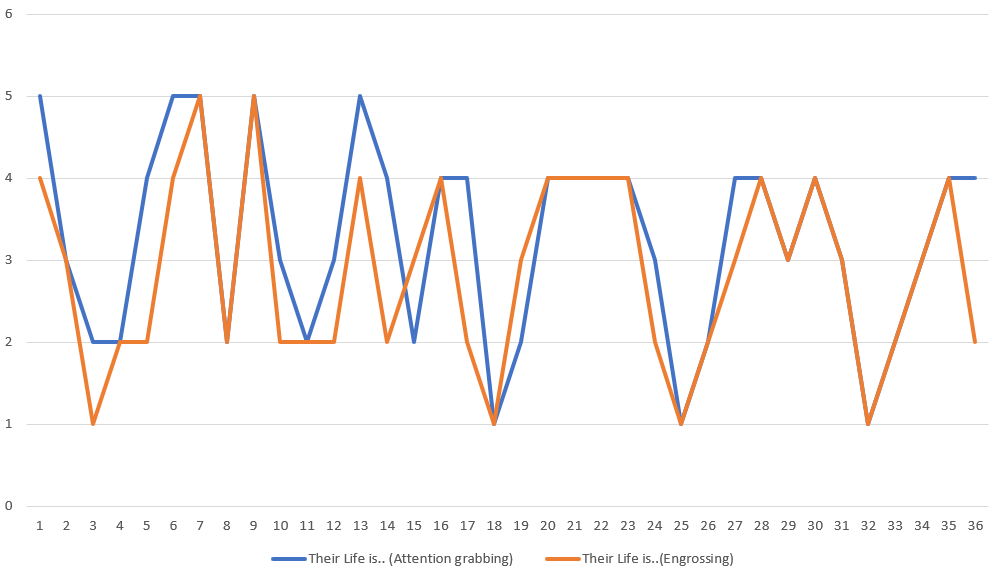
\includegraphics[scale=0.75]{Attention Grabbing vs Engrossing.png}
\end{figure}


\begin{figure}[h]
\caption{Tenseness vs Attention Grabbing}
\label{tab:TensenessvsAttentionGrabbing}
 \centering
 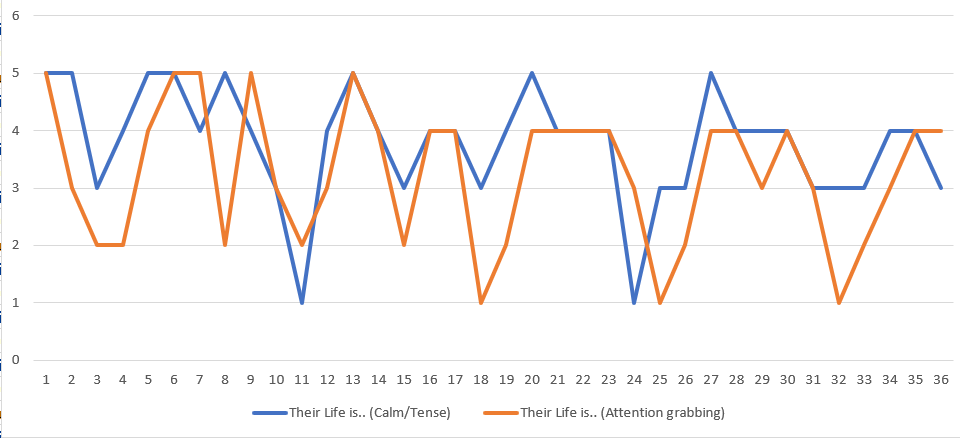
\includegraphics[scale=0.75]{Tenseness vs Attention Grabbing.png}
\end{figure}

\pagebreak

\begin{figure}[h]
\caption{Tenseness vs Engrossing}
\label{tab:TensenessvsEngrossing}
 \centering
 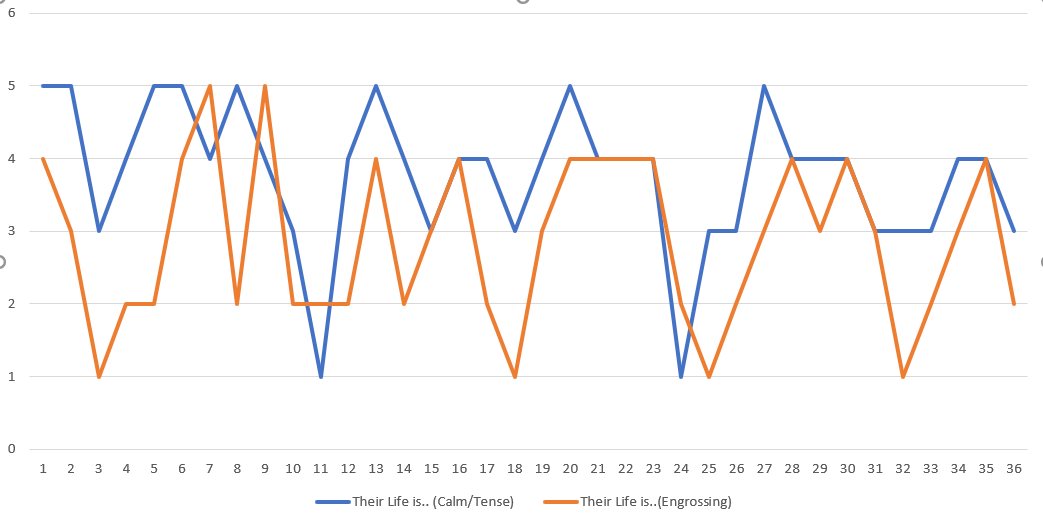
\includegraphics[scale=0.75]{Tenseness vs Engrossing.png}
\end{figure}

\begin{figure}[h]
\caption{Tenseness vs Entertaining}
\label{tab:TensenessvsEntertaining}
 \centering
 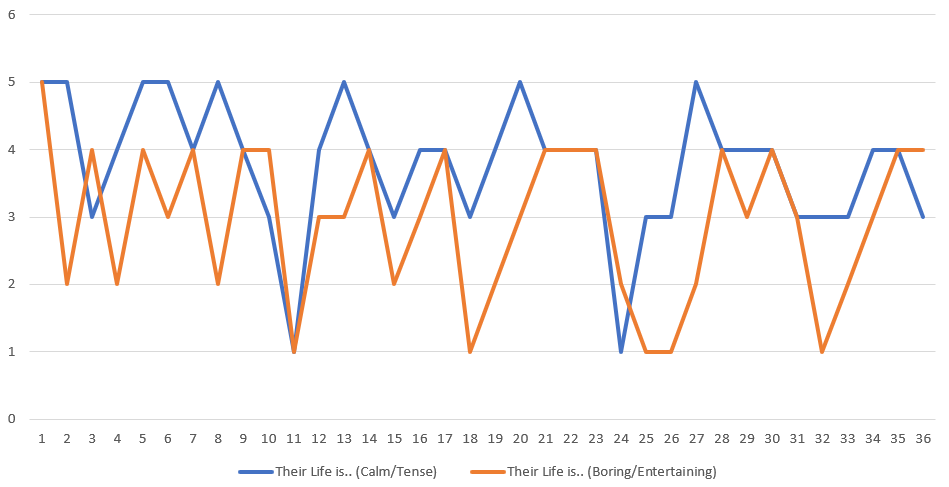
\includegraphics[scale=0.75]{Tenseness vs Entertaining.png}
\end{figure}

\pagebreak

\subsection{Decision Trees}

\begin{figure}[h]
\caption{First Method J48 First Data}
\label{tab:FirstMethodJ481}
 \centering
 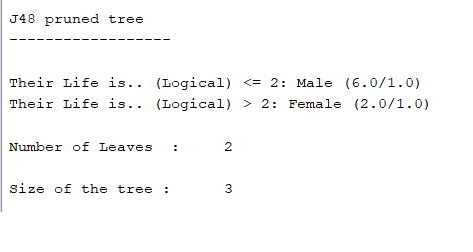
\includegraphics[scale=0.75]{First Method J48 1.png}
\end{figure}

\begin{figure}[h]
\caption{First Method J48 First Data}
\label{tab:FirstMethodJ481}
 \centering
 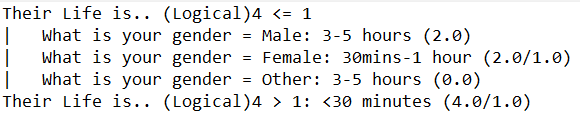
\includegraphics[scale=0.75]{First Method J48 2.png}
\end{figure}

\begin{figure}[h]
\caption{Second Method J48 First Data}
\label{tab:FirstMethodJ481}
 \centering
 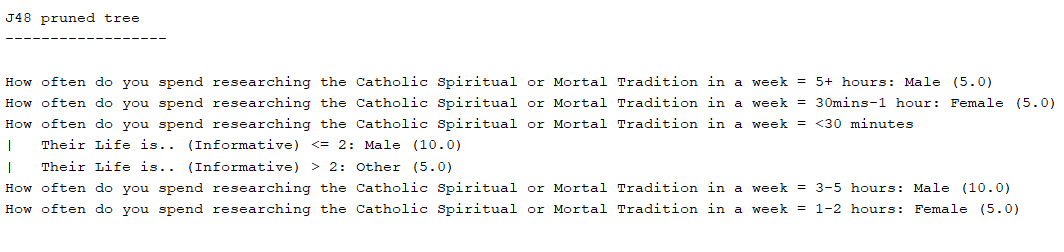
\includegraphics[scale=0.75]{Second Method J48 1.png}
\end{figure}

\end{document}

